\setlength\parindent{0pt}

\chapter{Battery Performace Testing}

\section{Setting up battery historian and UI Automator automation setup} Firstly, Battery Historian (a tool to analyze power use on Android devices, developed by Google) was setup on the given machine. ADB(Android Debug Bridge) was also set up for the purpose of generating battery statistics and bug reports. Following are the adb commands to use:\cite{adb}
\begin{lstlisting}[style=ShellStyle]
# to start the adb server
adb start-server

# to check connected devices
adb devices

# output of above command
# List of devices attached
# 02157df2d58dae03	device

#  find the IP address of device to connect to adb over WiFi
adb shell ip -f inet addr show wlan0

# output of above command
# 13: wlan0: <BROADCAST,MULTICAST,UP,LOWER_UP> 
#  mtu 1500 qdisc pfifo_fast state UP group default qlen 1000
#    inet 192.168.2.4/24 brd 192.168.2.255 scope global wlan0
#       valid_lft forever preferred_lft forever
# IP address is 192.168.2.4

# to use TCP for adb we have restart adb in TCPIP mode
adb tcpip 5555 # TCPIP port 5555

# connect to adb over WiFi
adb connect 192.168.2.4

# for resetting battery statistics
adb shell dumpsys batterystats --reset

# to take bugreport
adb bugreport bugreport.zip # for Android 7.0 Nougat and above
adb bugreport bugreport.txt # for Android versions prior to 7.0 

# to get batterystats file for a particular app 
# if the app package name is com.example.app
adb shell dumpsys batterystats com.example.app > batterystats.txt
\end{lstlisting}
These reports were to be analysed using Battery Historian. Android Studio, UIAutomator and other tools such as Apache Ant and Robot Framework were also setup .
\\

\section{Running UI Automator tests and understanding the flow} The existing test suite which is used in this project makes use of robot framework and UI Automator library. Hence learning to use these tools was an important part of the project. \\

\subsection{UI Automator} testing framework provides a set of APIs to build UI tests that perform interactions on user apps and system apps. The UI Automator APIs allows you to perform operations such as opening the Settings menu or the app launcher in a test device. The UI Automator testing framework is well-suited for writing black box-style automated tests, where the test code does not rely on internal implementation details of the target app.\cite{uiautomator} \\

Citrix makes use of an open source python wrapper written for UI Automator. For UI Automator to work, an Android device has to be connected to the computer over adb via USB or WiFi. Since the project work deals with analysing battery performance, adb was used over TCP as connecting adb via USB will continuously charge the battery, which leads to these problems:
\begin{itemize}
	\item Charging the device leads to the batterystats data to be reset, hence information on battery usage patterns over the duration of the test is lost
	\item Even if the data was not lost, battery usage patterns will be erroneous if read from a device which is charging as gauing how much battery was actually consumed becomes difficult.
\end{itemize}	 

Some sample code on UI Automator workings:

\begin{lstlisting}[style=PyStyle]
# connecting to ui automator

from uiautomator import Device
d = Device('014E05DE0F02000E') # device serial number 
\end{lstlisting}

The device serial number is found after connecting the device to the computer and running the adb command `adb devices'. Device serial numbers for devices connected via USB are generally alphanumeric strings, while for devices connected over WiFi the serial numbers are the IP addresses of the device. Note that for adb to work over WiFi, both the device and the computer have to be connected to the same WiFi network

\begin{lstlisting}[style=PyStyle]
# retrieving device information
d.info 
\end{lstlisting}

A sample output for this could be as below:
\begin{lstlisting}[style=PyStyle]
{ u'displayRotation': 0,
  u'displaySizeDpY': 640,
  u'displaySizeDpX': 360,
  u'currentPackageName': u'com.android.launcher',
  u'productName': u'product',
  u'displayWidth': 720,
  u'sdkInt': 18,
  u'displayHeight': 1184,
  u'naturalOrientation': True
}
\end{lstlisting}

UI Automator is also being used to mock how an user would use the app. It is used to perform clicks and type in text fields. UI Automator makes use of selectors to identify UI elements on the screen. There are many times of selectors including:
\begin{itemize}
	\item resourceId, which is the ID of the UI element
	\item text, the text present in the UI element. We can also use textContains which finds elements which contain the text specified instead of looking for an exact match
	\item classname, which is the class of the UI element, such as TextView, ListView, etc
	\item Action based selectors such as checkable, checked, clickable, longClickable, scrollable, enabled,focusable, focused, selected
\end{itemize}
\begin{lstlisting}[style=PyStyle]
# sample code to perform a click
if device(text='OK').exists:
    device(text='OK').click()
\end{lstlisting}
Documentation for UIAutomator python wrapper can be found on GitHub. \cite{uiautomatordoc}\\

\subsection{Robot Framework} is a generic test automation framework for acceptance testing and acceptance test-driven development (ATDD). It has easy-to-use tabular test data syntax and it utilizes the keyword-driven testing approach. Its testing capabilities can be extended by test libraries implemented either with Python or Java, and users can create new higher-level keywords from existing ones using the same syntax that is used for creating test cases \cite{robot}.
A sample robot test case:
\begin{lstlisting}[style=PyStyle]
*** Test Cases ***
User can create an account and log in
    Create Valid User    fred    P4ssw0rd
    Attempt to Login with Credentials    fred    P4ssw0rd
    Status Should Be    Logged In

User cannot log in with bad password
    Create Valid User    betty    P4ssw0rd
    Attempt to Login with Credentials    betty    wrong
    Status Should Be    Access Denied
\end{lstlisting}

Robot Framework allows use of keywords, which can be python functions. We will be using such keywords for our purposes. A simple example is as follows:

\begin{lstlisting}[style=PyStyle]
def sample_test_case(d, username, password):
	if d(text='username'):
		d(text='username').set_text(username)
	if d(text='password'):
		d(text='password').set_text(password)
	if d(text='ok'):
		d(text='ok').click()	
# robot test case
Test username and password
  [Tags]    Test
  ${username}     User
  ${password}     Password
  Wait until keyword succeeds     2 min   0 sec   
  sample test case    ${device01}    ${username}     ${password}
\end{lstlisting}
After learning how to use these tools, simple test cases were written for the app the project involves. These test cases were solely written for the purpose of training and were not added to the actual code base. 

\section{Writing a shell script to send multiple emails} 
The task at hand was to write a script that sends a batch of 50 emails in half hour intervals, for a total of 150 mails over 1 and half hour. \\

\subsection{Approaches tried}

\subsubsection{Postfix:} Postfix is a free and open-source mail transfer agent that routes and delivers electronic mail. To learn the usage of Postfix, a simple Gmail relay was setup. This is the basic Postfix main configuration, which needs to be added at the end of the Postfix main configuration file (usually found at /etc/postfix/main.cf on UNIX based systems)

\begin{lstlisting}[style=ShellStyle]
mail_owner = _postfix
setgid_group = _postdrop
relayhost = smtp.gmail.com
\end{lstlisting} 

Most mail servers use SASL (Simple Authentication and Security Layer). Hence we need to configure postfix to enable SASL. This can be done by adding the following lines to the end of the Postfix main configuration file. 

\begin{lstlisting}[style=ShellStyle]
smtpd_sasl_auth_enable = yes
smtp_sasl_auth_enable = yes
smtp_sasl_password_maps = hash:/etc/postfix/sasl/sasl_passwd
smtp_sasl_security_options = noanonymous
smtp_sasl_mechanism_filter = plain
\end{lstlisting}

At line 3 above, the file used for sasl authentication is specified. File contents:
\begin{lstlisting}[style=ShellStyle]
smtp.gmail.com username:password
\end{lstlisting}

Gmail additionally requires TLS (Transport Layer Security) to be configured
\begin{lstlisting}[style=ShellStyle]
smtp_use_tls = yes
tls_random_source = dev:/dev/urandom
smtp_tls_mandatory_ciphers = high
smtp_tls_security_level = secure
compatibility_level = 2
\end{lstlisting}
This is based on an article found on HowtoForge \cite{postfix}\\

Compatibility level causes Postfix to run with backwards-compatible default settings after an upgrade to a newer Postfix version \cite{compatibility}. By default, it is set to 0 to enable backwards compatibilty. But the default setting was causing issues with the working of Postfix. Hence it was set to 2, to disable backwards compatibilty, as suggested by the error trace.\\

To run Postfix, first a Postfix lookup table must be generated by using the following command:
\begin{lstlisting}[style=ShellStyle]
postmap /etc/postfix/sasl/sasl_passwd
\end{lstlisting} 
Then the Postfix service has to be started:
\begin{lstlisting}[style=ShellStyle]
service postfix start
\end{lstlisting}
Finally we can use this relay to send emails:
\begin{lstlisting}[style=ShellStyle]
echo "This is a test." | mail -s "test message" user@mail.com
\end{lstlisting}
NOTE: To send emails using this relay, the sender must allow less secure apps to access gmail, which can be done from gmail settings.\\

Although this worked with the gmail SMTP, due to network restrictions on company network, Postfix could not connect to the internal mail servers, leading to an 'Operation Timed Out' error\\

\subsubsection{msmtp:} msmtp is a mail client similar to Postfix. msmtp also needs to be configured. The follwing is a sample configuration file (the file is named msmtprc) \cite{msmtp}

\begin{lstlisting}[style=ShellStyle]
defaults
tls on
tls_starttls on
tls_trust_file /etc/ssl/certs/certificate.crt
account default
host ""
port 25
auth on
user ""
password ""
from ""
\end{lstlisting}
msmtprc permissions must be changed to make it executable. This cane be done by using the following command:
\begin{lstlisting}[style=ShellStyle]
chmod +x msmtprc
\end{lstlisting}
msmtp usage is pretty similar to Postfix 
\begin{lstlisting}[style=ShellStyle]
echo "This is a test." |msmtp -t user@mail.com
\end{lstlisting}
However, since the issue was with the network settings for the company network, msmtp did not work either. Hence, this task was suspended and work was moved on to the next task.\\

\section{Segregating the Test Cases (TCs) which test most commonly used UI interactions and add TAG as `BatteryPerf'} The UI Automation Suite already had test cases for almost all functionality available in the app. The task at hand was to pick test cases which test UI actions which are commonly performed by users. The test cases included Build Validation Test (BVT) cases and Function Validation Test (FVT) cases.  \\
To get this done, first and foremost the flow of work of the automation suite  had to understood. The flow of code execution is as follows: 
\begin{enumerate}
	\item Build and run the MainDriver using Gradle
	\begin{lstlisting}[style=ShellStyle]
	./gradlew build && ./gradlew run
	\end{lstlisting}
	The MainDriver consists of all the arguments needed to run the tests. This file is used in the Jenkins automation server to run the automation process.
	\item The MainDriver calls a shell script which sets all the arguments passed to the MainDriver as environment variables in a subshell, which are then used by robot framework when running the robot test cases.
	\item The shell script sets the environment variables and starts the robot test cases.
	\item Robot Framework runs all test cases which contain the tag specified and generates reports.
\end{enumerate}
The code was run, but a few issues arised the first few times. Listed below are some problems faced:
\begin{itemize}
	\item Navigating through the very deep levels of industrial level project folder can be confusing at first.
	\item Since the MainDriver is used by Jenkins, where the arguments needed to be passed to the shell script are provided externally, the args[] array was commented out. To run the code locally this line needed to be uncommented, which was not done due to lack of knowledge about the same. So since the shell script was being called without any arguments, no environment variables were being set and robot tests did not run.
	\item When the args[] array was uncommented, robot framework showed 0 test cases passed, 0 test cases failed. Trying to figure why this was happening, the environment variables were looked at and it was observed that they were not set, making it the potential reason for the above reason. In order to fix this the environment values were set manually, which interfered with some of the system's necessary variables, leading to issues with the OS, and the machine had to be given to the IT services for reimaging. The variables are to be set for a session of a subshell, to be used by robot framework and not at system level.
\end{itemize}

Due to these issues, a demonstration was done by the guides on how exactly the test suite is to be run, and how to troubleshoot issues. \\

Post learning how to run the test suite, the next job was to look into the test cases in the BVT and FVT files to determine which test cases would be appropriate to run for battery performance analysis. The original shortlist had 20 test cases, but this list had to be further restricted to 10-12 test cases. In the end, the final shortlist had 12 test cases and the tag `BatteryPerf' was added to these test cases. Now by specifying `BatteryPerf' as the tag in the MainDriver file, the battery performance test could be run.\\

The report generated for the tests are shown in tables 4.1, 4.2 and 4.3.

\begin{table}[!h]
\begin{center}
\caption{General Statistics}
\label{my-label}
\begin{tabular}{|P{8cm}|P{6.5cm}|}
\hline
Device estimated power use                  & 0.36\%                      \\ \hline
Foreground                                  & 156 times over 27m 5s 614ms \\ \hline
CPU User Time                               & 4m 25s 40ms                 \\ \hline
CPU System Time                             & 1m 42s 130ms                \\ \hline
Device estimated power use due to CPU usage & 0.0\%                       \\ \hline
Total number of wakeup alarms               & 20     \\    \hline                
\end{tabular}
\end{center}
\end{table}

\begin{table}[!h]
\begin{center}
\caption{Sync Information}
\label{my-label}
\begin{tabular}{|P{4cm}|P{4cm}|P{4cm}|}
\hline
Sync Name        & Time (ms) & Count \\ \hline
Tasks Provider   & 566       & 1     \\ \hline
Note Provider    & 399       & 1     \\ \hline
Android Contacts & 392       & 1    \\ \hline
\end{tabular}
\end{center}
\end{table}
\pagebreak

\begin{table}[!h]
\begin{center}
\caption{Service Information}
\begin{tabular}{|P{7cm}|P{3cm}|P{2cm}|P{2cm}|}
\hline
Service Name                      & Time          & Starts & Launches \\ \hline
ExchangeService                   & 30m 19s 270ms & 8      & 25       \\ \hline
EmptyService                      & 1m 12s 846ms  & 20     & 21       \\ \hline
AttachmentDownloadService         & 11s 616ms     & 27     & 27       \\ \hline
PDLIntentService                  & 7s 360ms      & 19     & 19       \\ \hline
MailService                       & 6s 843ms      & 16     & 16       \\ \hline
FCMService                        & 2s 859ms      & 1      & 1        \\ \hline
ContactSaveService                & 324ms         & 2      & 2        \\ \hline
CalendarProviderIntentService     & 168ms         & 2      & 2        \\ \hline
AsyncQueryServiceHelper           & 120ms         & 2      & 2        \\ \hline
ExchangeBroadcastProcessorService & 59ms          & 1      & 1        \\ \hline
EmailBroadcastProcessorService    & 43ms          & 1      & 1        \\ \hline
AccountService                    & 0ms           & 0      & 48       \\ \hline
EasAuthenticatorService           & 0ms           & 0      & 1        \\ \hline
PolicyService                     & 0ms           & 0      & 19       \\ \hline
LocalContactsSyncAdapterService   & 0ms           & 0      &  1        \\ \hline
NoteSyncAdapterService            & 0ms           & 0      & 1        \\ \hline
CtxAppManager                     & 0ms           & 0      & 17       \\ \hline
\end{tabular}
\end{center}
\end{table}

This information was obtained from Battery Historian\\

When running the test cases, it was observed that for some cases emails were being sent to the test account. These emails were sent using the Java Exchange Web Services API and a corresponding Python wrapper. The feasibility of using these APIs to send the batch mails was looked into and since it was feasible, code was added for sending the batch emails. A corresponding test case was also added to the robot test cases file to send and verify batch emails. During developing this test case, one problem faced was that during the 30 minute intervals between mail batches, since the phone was idle, the phone would go to Android Doze mode, which led to adb over WiFi disconnecting. To solve this issue, the device was polled once every minute to ensure that it does not go into doze mode. Although this is a deviation from a practical use point, this was necessary to run tests, and the polling hardly affected the battery usage as it does not do any computation that may require CPU or network usage. This test was primarily to check battery performance for sync operations. Results for this test are illustrated in tables 4.4 and 4.5.

\begin{table}[!h]
\begin{center}
\caption{General Statistics}
\begin{tabular}{|P{8cm}|P{6.5cm}|}
\hline
Device estimated power use                  & 0.05\%                      \\ \hline
Foreground                                  & 0 times over 1hr 42m 16s 412ms \\ \hline
CPU User Time                               & 22s 30ms                 \\ \hline
CPU System Time                             & 13s 934ms                \\ \hline
Device estimated power use due to CPU usage & 0.0\%                       \\ \hline
Total number of wakeup alarms               & 0     \\    \hline                
\end{tabular}
\end{center}
\end{table}

\begin{table}[!h]
\begin{center}
\caption{Service Information}
\begin{tabular}{|P{7cm}|P{3cm}|P{2cm}|P{2cm}|}
\hline
Service Name                      & Time          & Starts & Launches \\ \hline
ExchangeService                   & 16m 40s 282ms & 1      & 1       \\ \hline
EmptyService                      & 1s 8ms  & 1     & 1       \\ \hline
AttachmentDownloadService         & 430ms     & 1     &1       \\ \hline
MailService                  & 413ms      & 1    & 1       \\ \hline
PDLIntentService                       & 284ms      & 1     & 1       \\ \hline
AccountService                    & 0ms           & 0      & 2       \\ \hline
PolicyService                     & 0ms           & 0      & 1       \\ \hline
CtxAppManager                     & 0ms           & 0      & 1       \\ \hline
\end{tabular}
\end{center}
\end{table}

It can be seen from this even though the batch email sync test case ran for a longer time, the device and the application, apart from running the sync service, were mostly idle and hence the battery consumption is minimal.\\

From the reports of the BVT and FVT test cases, it can be observed that the Attachment Download Service is running a large number of times (27), even though there were only two test cases that needed to use this service. This behaviour seemed erroneous and had to be looked into, to figure what was causing this issue. After looking into the source code, excessively logging the workflow of attachment download and consulting the original author of the code, following was learnt:
\begin{itemize}
	\item The service is run once every time the app is launched, to check if any of the emails have an attachment, and to auto download the attachment, if auto download is enabled
	\item The service is also responsible for inline attachment download, and not just file attachments
\end{itemize}
This justified the large number of starts for the service. It was also learnt that the auto download feature only worked when the device memory was less than 75\% full. Next, a test was perofrmed to check if indeed the auto download behaviour was behaving as intended. To do this, a simple C program was written to allocate large amounts of memory to the program. While doing this a cross compiler, the ARM Cross Compiler for Android to be precise, needed to be used as C programs are platform dependent, and hence a program compiled on a computer will not run on the phone.\\

To compile and run a C program on an Android device, we can follow the following steps:
\begin{lstlisting}[style=ShellStyle]
#compile using ARM Cross Compiler
arm-linux-gnueabi-gcc -static -march=armv7-a test.c 
#push generated file to device
adb push a.out /data/local/tmp/.
#run the program
adb shell "./data/local/tmp/a.out"  
\end{lstlisting}
After filling the memory, two attachment test cases were run and the auto download behaviour was as expected.Auto download only worked when memory was more than 25\% empty.\\

Originally it was planned to run the entire battery performance test under low free memory conditions, but Android system automatically deallocates memory by shutting down background apps, processes and services when memory consumption becomes high, and hence the program could only keep the memory consumption high for the duration of the attachment tests, hence the entire battery performance test could not be run under low free memory conditions. \\

It was also planned to carry out the battery performance test under network fluctuations and also on 3G/4G network. But due to unavailability of a SIM card, and issues with creating network fluctuations, these tasks have been removed from the project.\\

\section{Creating a jenkins job and configure it to run Battery Performance automation}Jenkins is an open source automation server written in Java. Jenkins helps to automate the non-human part of software development process, with continuous integration and facilitating technical aspects of continuous delivery. The next task was to automate the entire battery performance test and to run it on the team Jenkins server, end to end without any manual work. For this the following needed to be done:
\begin{itemize}
	\item Learn how to work with Jenkins, and get familiar with it.
	\item Develop a simple reporting tool to report the battery usage patterns, as Battery Historian (used previously) has to be run manually, and is also very verbose, which makes it unsuitable for our purposes
	\item Create a Jenkins job and run it
\end{itemize}

So, a local Jenkins server was setup to see and learn the workings of Jenkins. By default a local Jenkins server runs at localhost:8080. When started for the first time, Jenkins needs to be unlocked using a password, which can be found on terminal which is running Jenkins on UNIX based systems.\\

Steps to create and run a Jenkins job:
\begin{enumerate}
	\item Create `new freestyle project' from the `create new jobs' option on the Jenkins dashboard and give it a name
	\item We need to specify the location of files which need to be built. Let's assume that a local git repository(/Users/user/Project) has been setup which contains a `HelloWorld.java' file. Select Git option and enter the URL of the local git repository. (We can also add the url of a remote git repository, or download and use the File System SCM plugin to directly use directories from the file system, which are not git repositories)
	\item In the build section, add build step. Since I am working on a UNIX based machine, I needed to select `Execute shell' option and add the command javac HelloWorld.java \&\& java HelloWorld
	\item Save and run the job
	\item Check the output, logs or errors on the console available in Jenkins
\end{enumerate}
Jenkins allows users to set parameters to be used as arguments while running a job. This will be used to supply arguments to the MainDriver program, instead of specifying the arguments in the MainDriver file itself, as this gives the flexibility to change any arguments if needed before every run. Jenkins also allows setting of build and job run triggers. One such trigger could be committing code to the git repository associated with the Jenkins job.

Moving on, a simple battery usage reporting tool was developed for automation purposes, as Battery Historian needs to be run manually and hence cannot be integrated into the Jenkins job, and tested. The tool reads the batterystats file and generated a HTML report showing wakelocks, wakeup alarms, jobs and syncs. The reporting tool takes either a single batterystats file or a text file containing a list of batterystats files as input. In case a list of batterystats files is supplied as input, a separate report is generated for every file. The script primarily performs text mining on the batterystats file and stores the required information in dictionaries. These dictionaries are then used to create tables and graphs. The reporter script reports job, service, sync and wakelock information Screenshots from the tool are shown in figures 4.1 and 4.2.\\
\begin{figure}[!h]
 	\begin{center}
		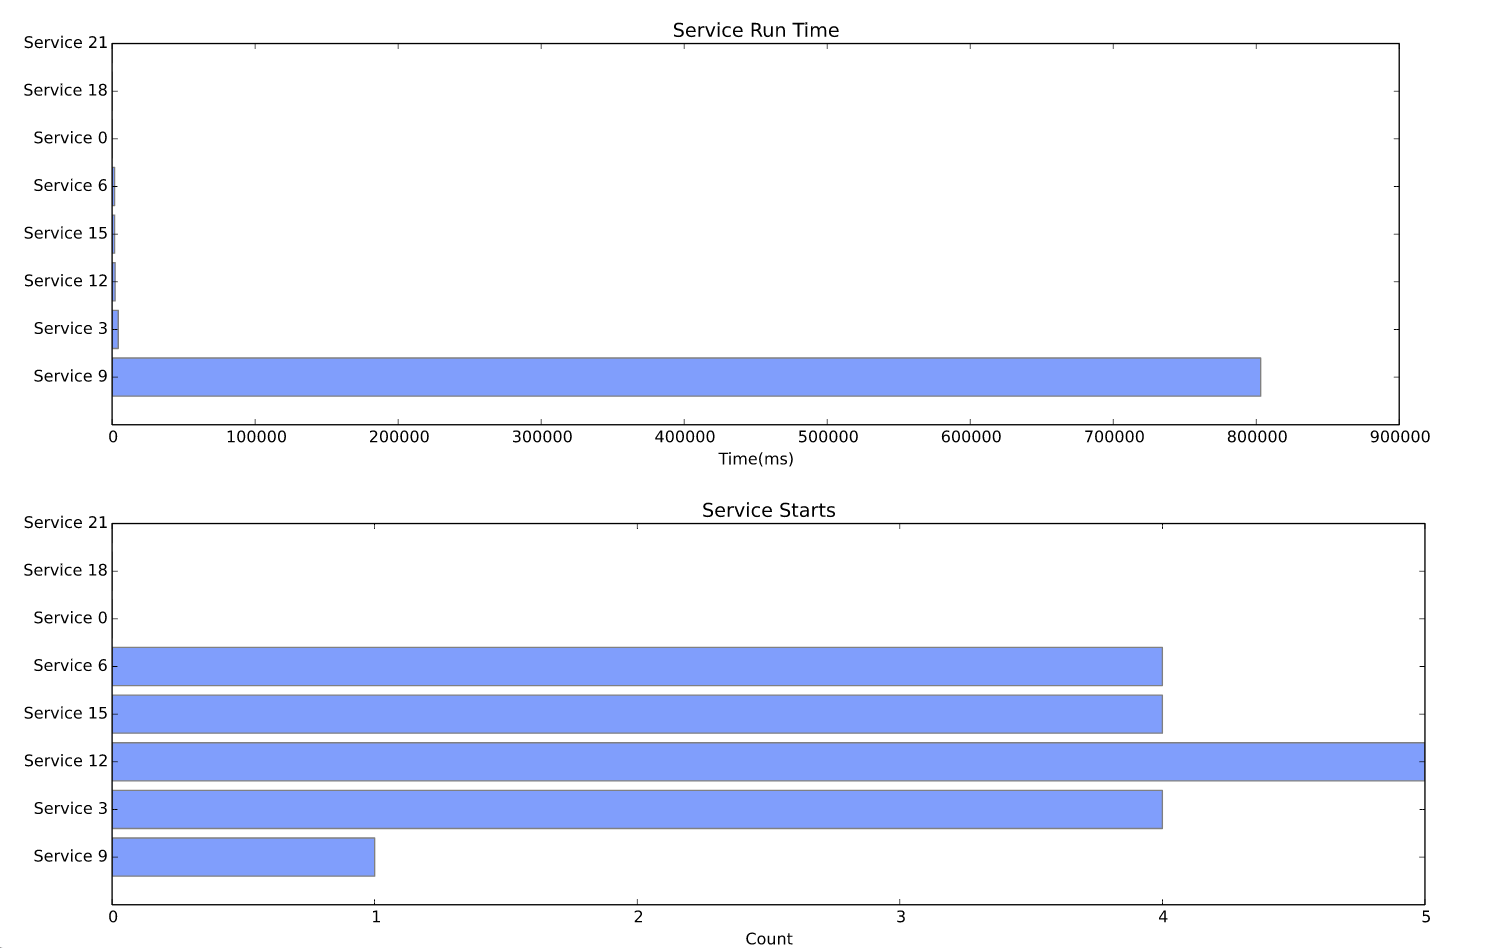
\includegraphics[scale=0.35]{reporter2}
		\caption{Service graphs}
		Similar graphs are generated for jobs, syncs and wakelocks
	\end{center}
\end{figure}
\begin{figure}[!h]
 	\begin{center}
		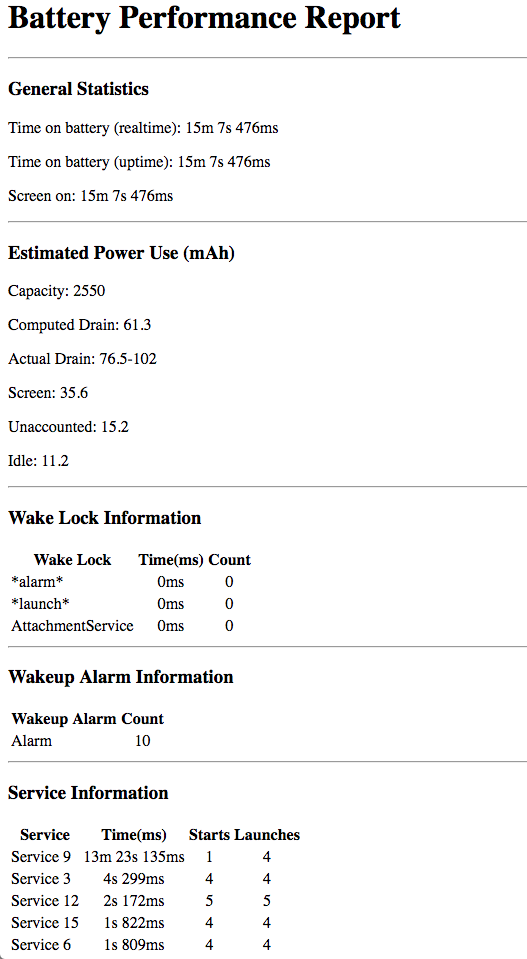
\includegraphics[scale=0.6]{reporter1}
		\caption{App Statistics}
	\end{center}
\end{figure}

After developing this reporting tool, the attachment download service was looked into again, to see if the large number of starts is consuming battery unnecessarily. To do this, two attachment test cases were added:
\begin{itemize}
	\item To send a number of mails with attachments in one go, and then open the app and open the mails one by one and download the attachments, as an user would when they receive multiple mails together.
	\item To alternately send and view the emails (Send one mail, open the mail, download attachment and then send next mail)
\end{itemize}
Test conditions:
\begin{itemize}
	\item Three cases were tested:
	\begin{itemize}
		\item Mails with no attachment
		\item Mails with a 133KB attachment
		\item Mails with a 1.4MB attachment
	\end{itemize}
	\item 20 mails were sent for every test case
\end{itemize}
\clearpage
\underline{Results for sending 20 mails in one go:} \\
\begin{table}[!h]
\centering
\caption{Battery Consumption}
\begin{tabular}{|c|c|}
\hline
Case & Battery Consumption\\ \hline
No Attachment & 0.20\%\\ \hline
133KB Attachment & 0.35\% \\ \hline
1.4MB Attachment & 0.34\% \\ \hline 
\end{tabular}
\end{table}
\begin{table}[!h]
\centering
\caption{Wakelock Count}
\label{my-label}
\begin{tabular}{|l|c|c|c|}
\hline
Wakelock                            & \multicolumn{3}{c|}{Start Count}                    \\ \hline
                                    & No Attachment & 133KB Attachment & 1.4MB Attachment \\ \hline
EmailSyncAlarmReceiver              & 20            & 20               & 20               \\ \hline
AttachmentDownloadWatchdog & 1             & 20               & 20               \\ \hline
\end{tabular}
\end{table}
\begin{table}[!h]
\centering
\caption{Service Running Time}
\label{my-label}
\begin{tabular}{|l|l|l|l|}
\hline
Service Name              & \multicolumn{3}{P{10cm}|}{Time}                           \\ \hline
                          & No Attachment & 133KB Attachment & 1.4MB Attachment \\ \hline
ExchangeService           & 19m 43s 830ms & 22m 53s 615ms    & 23m 19s 52ms     \\ \hline
AttachmentDownloadService & 1s 823ms      & 20s 355ms        & 36s 267ms        \\ \hline
EmptyService              & 4s 308ms      & 4s 59ms          & 4s 213ms         \\ \hline
PDLIntentService          & 2s 246ms      & 1s 976ms         & 2s 333ms         \\ \hline
MailService               & 1s 808ms      & 1s 534ms         & 1s 742ms         \\ \hline
\end{tabular}
\end{table}

\begin{table}[!h]
\centering
\caption{Service Start Count}
\label{my-label}
\begin{tabular}{|l|c|c|c|}
\hline
Service Name              & \multicolumn{3}{c|}{Start Count}                    \\ \hline
                          & No Attachment & 133KB Attachment & 1.4MB Attachment \\ \hline
ExchangeService           & 1             & 1                & 1                \\ \hline
AttachmentDownloadService & 4             & 99               & 106              \\ \hline
EmptyService              & 4             & 4                & 4                \\ \hline
PDLIntentService          & 7             & 6                & 4                \\ \hline
MailService               & 4             & 4                & 4                \\ \hline
\end{tabular}
\end{table}
\pagebreak
Observations: 
\begin{itemize}
	\item Since the app was opened only once, for the case with no attachments, the Attachment Download Service ran only once to check if there are any attachments. 
	\item With all other services running for same amount of time, it can be seen that increased running of the Attachment Download Service is a potential factor for the 0.15\% increase in battery consumption when downloading attachments. 
	\item The battery consumption might have also increased due to transfer of higher number of packets due to downloading of attachments, leading to higher network usage.
\end{itemize}
\underline{Results for sending and reading mails alternately: }\\
\begin{table}[!h]
\centering
\caption{Battery Consumption}
\begin{tabular}{|c|c|}
\hline
Case & Battery Consumption\\ \hline
No Attachment & 0.38\%\\ \hline
133KB Attachment & 0.45\% \\ \hline
1.4MB Attachment & 0.44\% \\ \hline 
\end{tabular}
\end{table}
\begin{table}[!h]
\centering
\caption{Wakelock Count}
\label{my-label}
\begin{tabular}{|l|c|c|c|}
\hline
Wakelock                            & \multicolumn{3}{c|}{Start Count}                    \\ \hline
                                    & No Attachment & 133KB Attachment & 1.4MB Attachment \\ \hline
EmailSyncAlarmReceiver              & 20            & 20               & 20               \\ \hline
AttachmentDownloadWatchdog & 1             & 20               & 20               \\ \hline
\end{tabular}
\end{table}
\begin{table}[!h]
\centering
\caption{Service Running Time}
\label{my-label}
\begin{tabular}{|l|l|l|l|}
\hline
Service Name              & \multicolumn{3}{P{10cm}|}{Time}                           \\ \hline
                          & No Attachment & 133KB Attachment & 1.4MB Attachment \\ \hline
ExchangeService           & 15m 55s 733ms & 19m 53s 615ms    & 21m 11s 931ms     \\ \hline
AttachmentDownloadService & 9s 418ms      & 28s 412ms        & 39s 842ms        \\ \hline
EmptyService              & 24s 31ms      & 26s 991ms          & 24s 303ms         \\ \hline
PDLIntentService          & 9s 423ms      & 10s 481ms         & 10s 781ms         \\ \hline
MailService               & 8s 108ms      & 10s 4ms         & 11s 27ms         \\ \hline
\end{tabular}
\end{table}

\begin{table}[!h]
\centering
\caption{Service Start Count}
\label{my-label}
\begin{tabular}{|l|c|c|c|}
\hline
Service Name              & \multicolumn{3}{c|}{Start Count}                    \\ \hline
                          & No Attachment & 133KB Attachment & 1.4MB Attachment \\ \hline
ExchangeService           & 1             & 1                & 1                \\ \hline
AttachmentDownloadService & 22             & 121               & 139              \\ \hline
EmptyService              & 22             & 24                & 24                \\ \hline
PDLIntentService          & 22             & 26                & 24                \\ \hline
MailService               & 22             & 24                & 24                \\ \hline
\end{tabular}
\end{table}
\pagebreak
Observations: 
\begin{itemize}
	\item The app was launched, the mail read, attachment downloaded and then closed for every mail, the Attachment Download Service ran 22 times even for the case with no attachments, once every time the app was launched. 
	\item With all other services running for same amount of time, it can be seen that increased running of the Attachment Download Service is a potential factor for the 0.06\% increase in battery consumption when downloading attachments. 
	\item The battery consumption might have also increased due to transfer of higher number of packets due to downloading of attachments, leading to higher network usage.
\end{itemize}

Among the items in the original project specification, was the development of user profiles for three types of users, namely heavy users, moderate users and light users. For this a script was written which can be run against a Microsoft Exchange server and will return the count of attachments (both file and inline) and appointments for the past one month, as well as the number of contacts. This will be done using either the Java Exchange Web Service (EWS) API or the Python exchangelib EWS API. The script automatically mails the counts to an email as attachments, with a common subject. The script was to be run against exchange accounts of volunteers to gather the data. Once the mails were, another script will be run against the MS Exchange Account which received the mails containing the information, to download all the data, and consolidate them into three files, one each for attachment data, appointment data and contact data, post which a clustering algorithm was to be run on these files, to find the centers for three clusters, which will be determine the average attachment, appointment and contact count for the three types of users. However it was realized that this approach would be highly erroneous as it would provide usage details of the user accounts in general and not on the app level, as this would account all attachements, contacts or appointments a user receives or creates irrespective of whether the client used (mobile app, desktop app, web app). Since the project required only the statistics of mobile app, and since there was no way to aggregate statistics of only the mobile app, it was decided to go with a relative comparison, wherein we would test every version of the app against a fixed arbitrary user profile\\

\section{Automating the entire process} The entire test will be run as a Jenkins job. This will consist of the following steps:
\begin{enumerate}
	\item Run specific BatteryPerf tests
	\item Run Email Sync Script
	\item Generate battery stats report and dump it in Jenkins archive
	\item Compare battery stats reports for different versions to check for improvements/deteriorations in battery performance, and dump comparision report to Jenkins archive

\end{enumerate}
To compare battery stats reports another script was developed, which makes use of the reporter script to generate the dictionaries. Then it compares the dictionaries and generates graphs for the differences. Screenshots of this tool can be seen in figures 4.3 and 4.4.
\begin{figure}[!h]
 	\begin{center}
		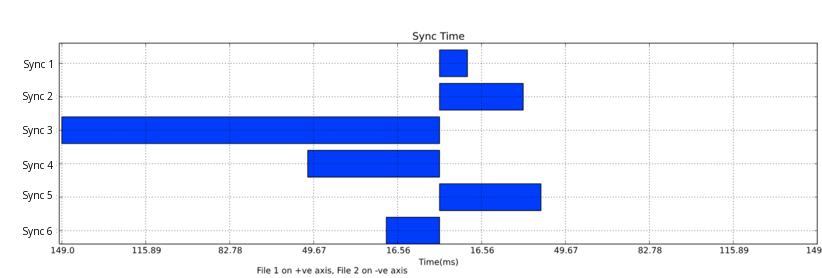
\includegraphics[scale=0.5]{diff2}
		\caption{Sync Difference Graph}
		Similar graphs are generated for jobs, services and wakelocks
	\end{center}
\end{figure}
\begin{figure}[!h]
 	\begin{center}
		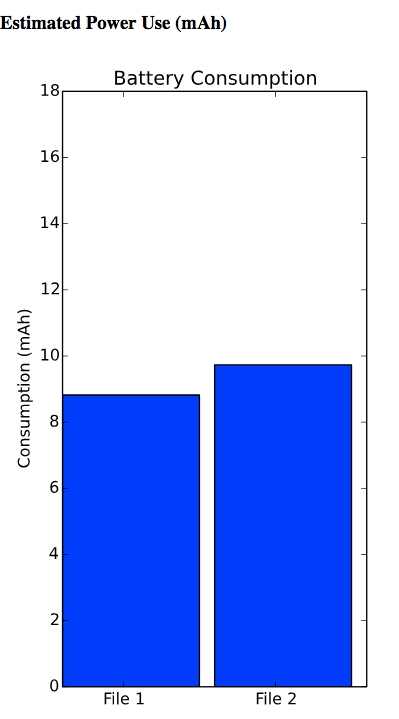
\includegraphics[scale=0.6]{diff1}
		\caption{Overall Battery Usage}
	\end{center}
\end{figure}

